Next, we built the whole mixing console and tested it.
\phantom{ } We combined all the parts we had built in previous labs, in the order of signal sources, (one of which was a microphone and preamplifier,) summing amplifier, equalizer, and speaker. The whole circuit graph is shown in the figure[\ref{fig:fullcir}]. 

\begin{figure}[!htbp]
	\centering
	\begin{framed}
		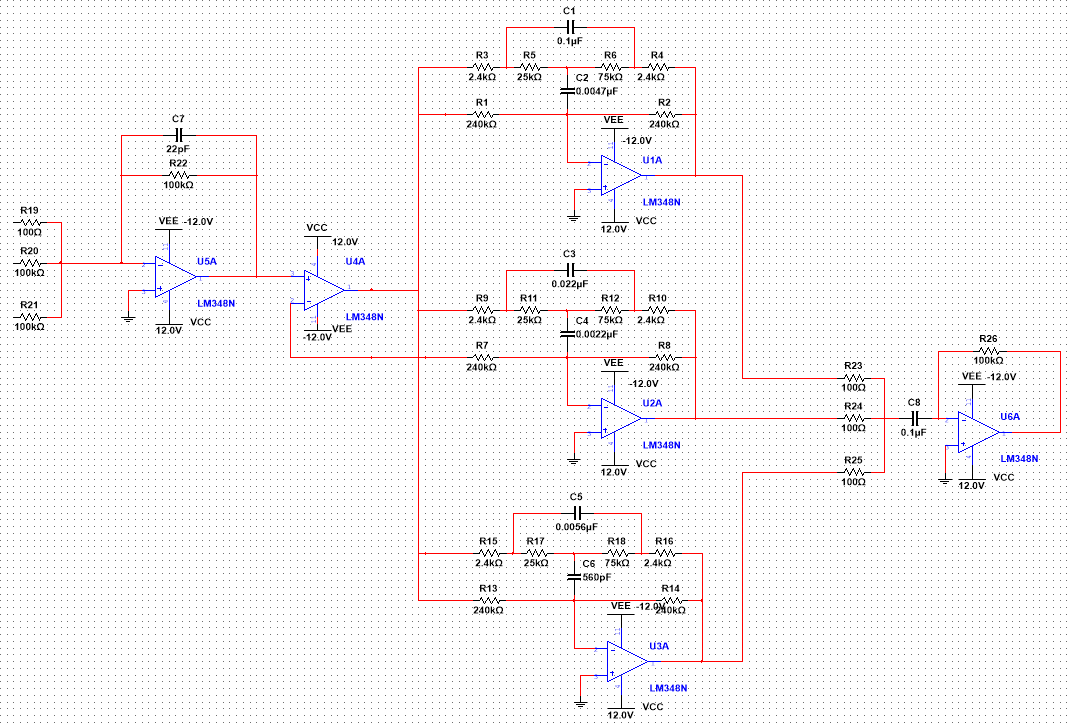
\includegraphics[width=\linewidth]{images/circ2.png}
		\caption{The audio mixer circuit}
		\label{fig:fullcir}
	\end{framed}
\end{figure}

\phantom{ } Then we used a sine wave of 250Hz as an input to the system. The waveform of the input and output signals are shown in figure[\ref{fig:wave250}].

\begin{figure}[!htbp]
	\centering
	\begin{framed}
		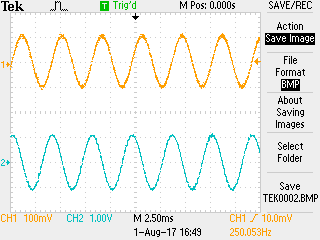
\includegraphics[width=\linewidth]{images/TEK0002.png}
		\caption{The waveform of the input and output signals}
		\label{fig:wave250}
	\end{framed}
\end{figure}

\phantom{ } To determine which filter controls the amplitude of the output at 250Hz, we changed each of the potentiometers of the three filters. While two of them did not make any change to the output wave form, when we adjusted $R_23$ to a lower resistance, the amplitude increased obviously. Since we only changed $R_23$, we can tell that the filter on the top of figure[\ref{fig:fullcir}] controls the output at 250Hz, as expected. Since the 250Hz case overlaps with the requirement of a waveform above, more evidence is provided in the cases below.

\phantom{ } Next, we used an input signal of 1kHz, and proved that the second filter controls the amplitude at this frequency. As the resistance of $R_24$ decreased, the amplitude of the output signal increased. The three figures below show the change of output signal when the potentiometer was at 100\%, 50\% and 0\%. Meanwhile, changing $R_23$ or $R_25$ did not make any difference to the waveform.

\begin{figure}[!htbp]
	\centering
	\begin{framed}
		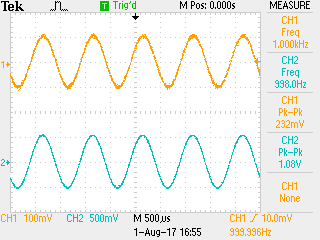
\includegraphics[width=\linewidth]{images/TEK0003.png}
		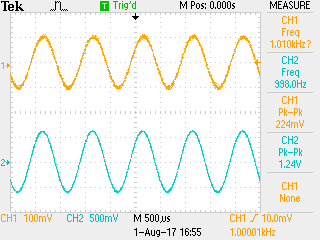
\includegraphics[width=\linewidth]{images/TEK0004.png}
		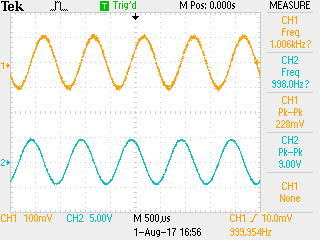
\includegraphics[width=\linewidth]{images/TEK0005.png}
		\caption{The changing of output signal at 1kHz}
		\label{fig:wave1k}
	\end{framed}
\end{figure}